\documentclass[12pt]{article}
\usepackage{amsmath,amssymb,amsthm}
\usepackage{graphicx,mathabx}
\usepackage{xcolor}
\usepackage{tikz}
\usepackage{soul}
\usepackage{placeins}
\usepackage{lipsum}
\usepackage{mathtools}
\usepackage[shortlabels]{enumitem}
\usepackage{wrapfig}
\DeclarePairedDelimiter{\ceil}{\lceil}{\rceil}
\begin{document}
\title{TCSS 343 - Week 2 - Wednesday}
\author{Jake McKenzie}
\maketitle
\noindent\centerline{\textbf{Asymptotics with an Introduction to the Analysis of Algorithms}}\\\\\\\\\\\\\\\\
\begin{center}
    ``There is nothing radical about moral clarity". \\$\cdots$\\ Alexandria Ocasio-Cortez
\end{center}
\begin{center}
    ``I am incapable of conceiving infinity, and yet I do not accept finity. I want this adventure that is the context of my life to go on without end". \\$\cdots$\\ Simone de Beauvoir
\end{center}
\begin{center}
    ``Man has not given himself the taste for the infinite and the love of what is immortal. These sublime instincts do not arise from a caprice of the will; they have their unchanging foundation in his nature; they exist despite his efforts. He can hinder and deform them, but not destroy them."\\
    $\cdots$\\
    Alexis de Tocqueville
\end{center}
\newpage
\begin{enumerate}
\item[0. ] Prove the theorem below using the techniques of binding the term and splitting the
sum to find a tight bound for the sum. Make sure your proof is complete, concise, clear
and precise.\\
\textbf{Theorem 0: }
$$\sum\limits_{i=1}^{n}i^4\in\Theta(n^5)$$
\newpage
\item Prove the theorem below using the techniques of binding the term and splitting the
sum to find a tight bound for the sum. Make sure your proof is complete, concise, clear
and precise.\\
\textbf{Theorem 1: }
$$\sum\limits_{i=1}^{n}(\log_2{i})^2\in\Theta(n(\log_2{n})^2)$$
\newpage
Here is an algorithm for singing that annoying song ``99 Bottles of Beer on the Wall''.
It exhibits all the qualities we expect from algorithms, namely that it is explicit, 
precise, unambiguous, mechanically-executable sequence of elementary instructions intended to 
accomplish a specific purpose.\\
\centerline{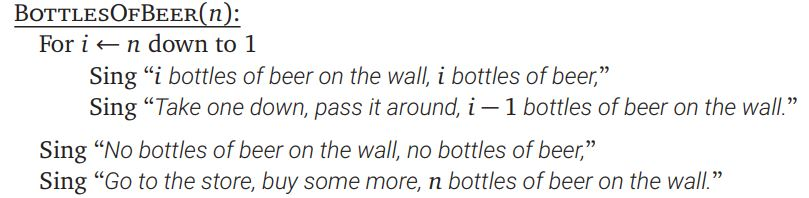
\includegraphics[scale = .6]{BoBeer.JPG}}\\
\item If you use this algorithm to sing this terrible song, $n$-times how many times will you say beer? $2n$? 
\newpage
Here is an algorithm for singing a far less annoying song, $12$ Days of Christmas, generalized to $n$ 
Days of Christmas. Instead of analyzing the exact \st{running} singing time, let focus on the asymptotic behavior. \\
\centerline{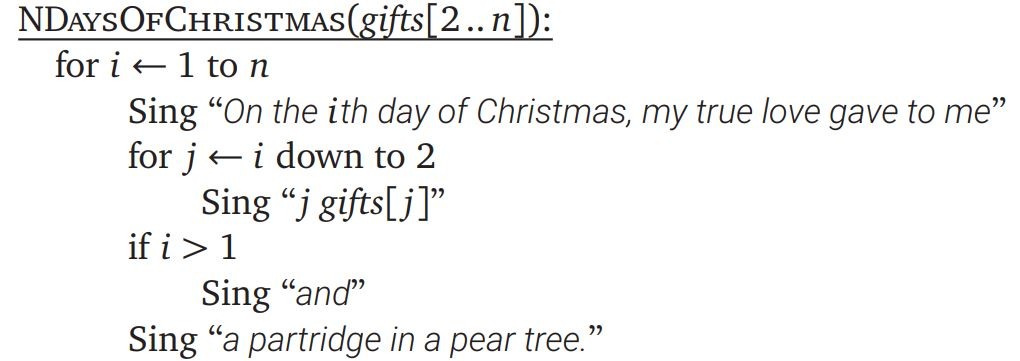
\includegraphics[scale = .5]{NDaysOfChristmas.JPG}}\\
\item How many gifts are sent into this algorithm? Express this as an exact answer.
\item During the first $n$ days of Christmas, my true love gate to me exactly how many gifts? Express 
this as a sum, then solve that sum finding the the big theta space complexity of the number of gifts my true love gave to me.
\newpage
\item Write does and solve the recurrence for the running time of an 
algorithm I've run into in the wild.\\
$$T(n)=3T(\frac{n}{4})+n^2$$
\newpage
\item Write does and solve the recurrence for the running time of the 
quickselect algorithm, used within quicksort.\\
$$T(n)=T(\frac{n}{3})+T(\frac{2n}{3})+n$$
\end{enumerate}
\end{document}










